\vspace{-0.5em}
\section{Data Filtering Details}
\label{ap:data_filtering_details}
In order to obtain high-quality training data, we designed a set of negative labels to filter out low-quality data. Figure \ref{fig:exp_filter} presents our negative labels along with sample videos for each label.In \cref{tab:classifier}, we present the accuracy and recall of our classifier, trained based on video-llama, on the test set (10\% randomly labeled data).

\begin{table}[h]
    \centering
    \caption{Summary of Classifiers Performance on the Test Set. TP: True Positive, FP: False Positive, TN: True Negative, FN: False Negative.}
        \begin{tabular}{cccccc}
        \toprule
        Classifier & TP  & FP & TN & FN & Test Acc \\
        \midrule
        Classifier - Editing & 0.81 & 0.02 & 0.09 &  0.08 & 0.91 \\ 
        Classifier - Static & 0.48 & 0.04 & 0.44 & 0.04 & 0.92 \\
        Classifier - Lecture & 0.52 & 0.00 & 0.47 & 0.01 & 0.99 \\
        Classifier - Text & 0.60 & 0.03 & 0.36 & 0.02 & 0.96 \\
        Classifier - Screenshot & 0.61 & 0.01 & 0.37 & 0.01 & 0.98 \\
        Classifier - Low Quality & 0.80 & 0.02 & 0.09 & 0.09 & 0.89 \\
        \bottomrule
        \end{tabular}
    \label{tab:classifier}
\end{table}

\begin{figure}[ht]
\begin{center}
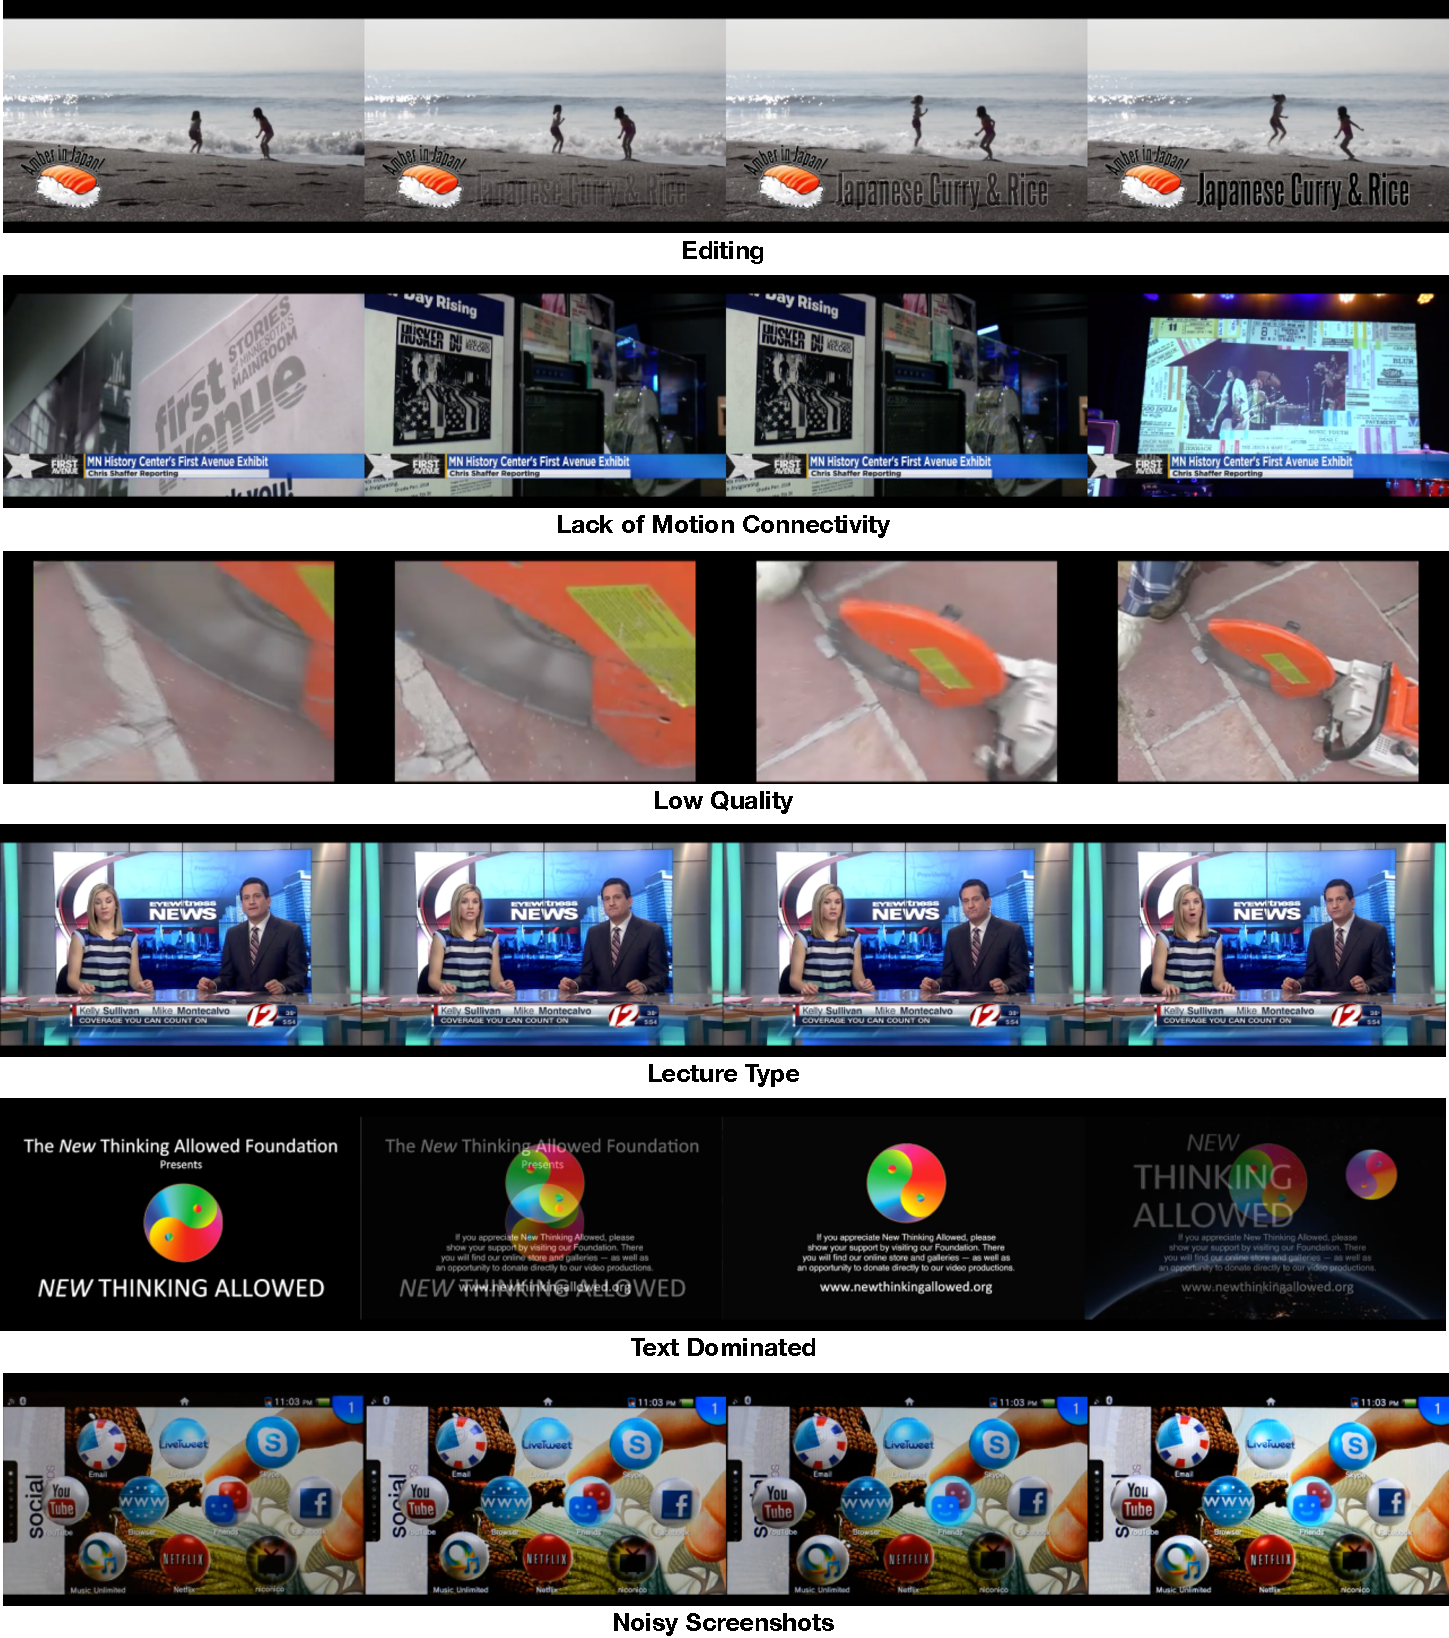
\includegraphics[width=0.9\linewidth]{images/data_filter/VideoFilter.pdf}
\end{center}
\vspace{-0.5em}
\caption{Examples of negative labels for video filtering.}
\label{fig:exp_filter}

\end{figure}

